\documentclass[a4paper]{oblivoir}
\usepackage{amsmath,amssymb,kotex,kswrapfig,mdframed,paralist}
\usepackage{fapapersize}
\usefapapersize{210mm,297mm,20mm,*,20mm,*}

\usepackage{tabto,pifont}
\TabPositions{0.2\textwidth,0.4\textwidth,0.6\textwidth,0.8\textwidth}
\newcommand\tabb[5]{\par\noindent
\ding{172}\:{\ensuremath{#1}}
\tab\ding{173}\:\:{\ensuremath{#2}}
\tab\ding{174}\:\:{\ensuremath{#3}}
\tab\ding{175}\:\:{\ensuremath{#4}}
\tab\ding{176}\:\:{\ensuremath{#5}}}

\usepackage{graphicx}

\pagestyle{empty}

%%% Counters
\newcounter{num}

%%% Commands
\newcommand\defi[1]
{\bigskip\par\noindent\stepcounter{num} \textbf{정의 \thenum) #1}\par\noindent}
\newcommand\theo[1]
{\bigskip\par\noindent\stepcounter{num} \textbf{정리 \thenum) #1}\par\noindent}
\newcommand\exam[1]
{\bigskip\par\noindent\stepcounter{num} \textbf{예시 \thenum) #1}\par\noindent}
\newcommand\prob[1]
{\bigskip\par\noindent\stepcounter{num} \textbf{문제 \thenum) #1}\par\noindent}

\newcommand\pb[1]{\ensuremath{\fbox{\phantom{#1}}}}

\newcommand\ba{\ensuremath{\:|\:}}

\newcommand\vs[1]{\vspace{40pt}}

\newcommand\an[1]{\bigskip\par\noindent\textbf{문제 #1)}\par\noindent}

%%% Meta Commands
\let\oldsection\section
\renewcommand\section{\clearpage\oldsection}

\let\emph\textsf

\begin{document}
\begin{center}
\LARGE준영, 미니테스트 09
\end{center}
\begin{flushright}
날짜 : 2017년 \(\pb3\)월 \(\pb{10}\)일 \(\pb{월}\)요일
,\qquad
제한시간 : \pb{17년}분
,\qquad
점수 : \pb{20} / \pb{20}
\end{flushright}

%
\prob{}
수열 \(\{a_n\}\)에서 첫째항부터 제 \(n\)항 까지의 합 \(S_n\)이 \(S_n=5^n+8\)일 때, \(\displaystyle\lim_{n\to\infty}\frac{S_n}{a_n}\)의 값을 구하여라.
\vs

%
\prob{}
아래 그림과 같이 자연수 \(n\)에 대하여 무리함수 \(y=\sqrt x\)의 그래프 위의 점 \(P_n(2n,\sqrt{2n})\)에서 \(x\)축에 내린 수선의 발을 \(Q_n\)이라 할 때, \(\displaystyle\lim_{n\to\infty}\left(\overline{OP_n}-\overline{OQ_n}\right)\)의 값을 구하여라.
(단, \(O\)는 원점)
\begin{figure*}[h!]
\centering
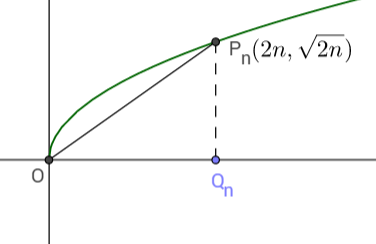
\includegraphics[width=0.25\textwidth]{sqrtx}
\end{figure*}
\vs


%
\prob{}
다음 세 수 \(A\), \(B\), \(C\)의 대소 관계를 바르게 나타낸 것은?
\begin{mdframed}
\(\displaystyle A=\lim_{n\to\infty}\frac{(-1)^n}{2n}\),
\qquad
\(\displaystyle B=\lim_{n\to\infty}\frac{5n}{\sqrt{n^2+4n}+n}\),
\qquad
\(\displaystyle C=\lim_{n\to\infty}\frac{3^n-2^n}{3^{n-1}+2^{n+1}}\)
\end{mdframed}
\tabb{A<B<C}{A<C<B}{B<A<C}{B<C<A}{C<A<B}
\vs

%
\prob{}
수열 \(\{a_n\}\)에 대하여 \(a_1=2\), \(a_2=2\sqrt2\), \(a_3=2\sqrt{2\sqrt2}\), \(\cdots\)일 때, \(\displaystyle\lim_{n\to\infty}a_n\)의 값은?
\tabb245{3\sqrt3}{4\sqrt3}
\vs

%
\prob{}
자연수 \(n\)에 대하여 \(6^n\)의 양의 약수의 총합을 \(a_n\)이라 할 때, \(\displaystyle\lim_{n\to\infty}\frac{a_n}{6^n}\)의 값은?
\tabb1{\frac32}23{\frac72}
\vs

\end{document}